\documentclass{ltjsarticle}
\usepackage{amsmath}
\usepackage{amssymb}
\usepackage{ascmac}
\usepackage[dvipdfmx]{graphicx}
\usepackage{tabularx}
\usepackage[colorlinks=true, allcolors=blue]{hyperref}
\usepackage{fancybox}
\usepackage{tikz}
\usepackage{subcaption}
\usetikzlibrary{shapes,arrows}

\begin{document}

\title{104. 深層学習の適用方法 (音声認識)}
\author{秋葉洋哉}
\maketitle

\section{音声認識}
\subsection{概要}
機械が音声を認識する技術を音声認識という。音声認識では音声信号を入力し、音声信号を認識しやすい表現に変換したのち、機械学習モデルに入力する。音声データを活用できるAIは、音声アシスタント、スマートスピーカー(一人ひとりの専用スピーカー)、自動議事録AIといった多様な形で活用されている。
音声認識をタスクとしたデータ分析コンペも多数存在し、これから発展していく分野と考えられる。
Kaggle Freesound Audio Tagging 2019では、短い音声データからギターや犬の鳴き声などにタグ付けするタスクのコンペであり、Kaggle BirdCLEF2021: Processing audio dataでは、鳥の鳴き声から鳥の種類を推測するタスクのコンペが開催されている。
\par
音声の振幅は音量、周波数は音の高さを表す。周波数がh[kHz]の音声を測定するには、最低2h[kHz]のサンプル数が必要になる。

\subsection{波形処理(特徴量抽出)}
横軸に時間、縦軸に振幅をとり、音声データをプロットしたものを波形という。音声データの波形には、周期的なものと、非周期的なものが存在する。そのうち、非周期的なものを、標本化、量子化、フーリエ変換といった波形処理を施すことで、様々な機械学習モデルに入力することができる。
\par
標本化とは、連続的な波形を離散的なデータに変換することである。量子化とは、波形の振幅を離散的な値に変換することである。

\subsection{フーリエ変換}
フーリエ変換とは、波形を周波数成分に分解する波形処理である。すなわち、ある波形$f(t)$から振幅・角周波数を表す関数$F(\omega)$に変換する作業と定義される(図\ref{fig:Fourier})。
\begin{figure}[htbp]
  \centering
  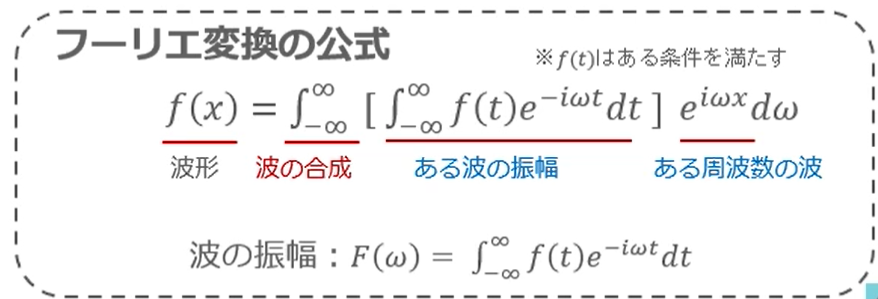
\includegraphics[width=10cm]{./capture/Fourier_def.png}
  \caption{フーリエ変換の定義}
  \label{fig:Fourier}
\end{figure}

\subsection{スペクトル}
スペクトルとは、波形の周波数成分を表すグラフである。周期的な波形をフーリエ変換した時、横軸を角周波数、縦軸を振幅としてグラフにプロットすると、離散的な周波数成分が得られる。これを離散スペクトルと呼ぶ。一方、非周期的な波形をフーリエ変換した時、横軸を周波数、縦軸を振幅としてグラフにプロットすると、連続的な周波数成分が得られる。これを連続スペクトルと呼ぶ。
\par
スペクトログラムは、スペクトルを利用した非周期音声データのグラフであり、音声データを横軸:時間と縦軸:周波数に分解したものある。窓関数を用いて、音声データを一定時間ごとに区切り、その区間ごとにフーリエ変換を行って、スペクトルにし、それを時間軸に沿って並べたものである(図\ref{fig:Spectrogram})。
\begin{figure}
  \centering
  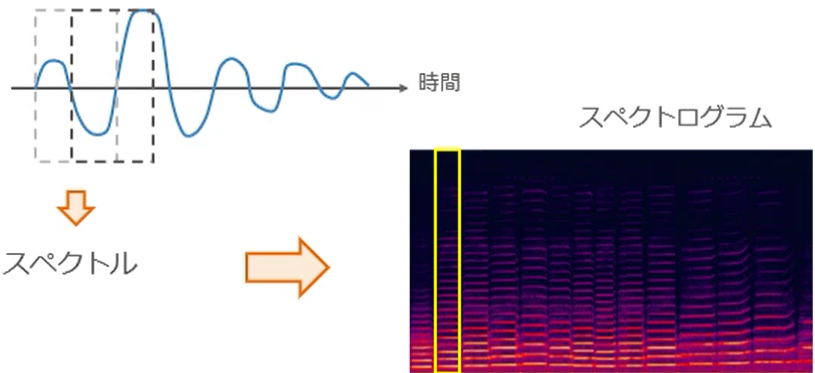
\includegraphics[width=10cm]{./capture/Spectrogram.png}
  \caption{スペクトログラムのプロット方法: 窓関数をズラしていき、明るさで振幅、色相で周波数を表す。窓関数によって、無限に分解可能な連続スペクトルを、ある程度の大きさに分割し、離散スペクトルとして表現しやすい形に分解する。}
  \label{fig:Spectrogram}
\end{figure}
\par
窓関数は、周期波であれば、矩形窓を採用しても問題はない。矩形窓は、0-1の値を持ち、窓の端で急激に0になる。
\begin{align}
  w(n) = 
  \begin{cases}
    1 & (0 \leq n \leq N-1)\\
    0 & (\text{otherwise})
  \end{cases}
\end{align}
これは、周期波であれば、窓関数の切り出す波形が周期的であるため、周期拡張したときにうまく波形がつながるからである。
\par
しかし、非周期波の場合、窓関数の切り出す幅$N$を決めて周期拡張したときに、つなぎ目が綺麗につながるとは限らない。うまい$N$を選ぶということは不可能に近い。そのため、非周期波の場合は、ハミング窓を用いることが一般的である。ハミング窓は、0-1の値を持ち、窓の端で滑らかに0になるような関数である。
\begin{align}
  w(n) =
  \begin{cases}
    0.54 - 0.46\cos\left(\frac{2\pi n}{N-1}\right) & (0 \leq n \leq N-1)\\
    0 & (\text{otherwise})
  \end{cases}
\end{align}
ハミング窓は両端で滑らかに0になるため、周期拡張してもつなぎ目が綺麗につながる。そのため、非周期波の場合は、ハミング窓を用いることが一般的である。



\subsection{DFT}
離散フーリエ変換(DFT)は、離散的な波形を周波数成分に分解する波形処理である。DFTは、離散的な波形$f(t)$から振幅・角周波数を表す関数$F(\omega)$に変換する作業である。DFTは、離散的な波形を周波数成分に分解するため、音声データを機械学習モデルに入力する際に用いられる。

\subsection{FFT}
高速フーリエ変換(FFT)は、DFTを高速に計算するアルゴリズムである。
窓のサンプルのうち、偶数番目と奇数番目をそれぞれ分けて、それぞれのDFTを計算することで、計算量を削減する手法である。FFTは、DFTの計算量が$O(n^2)$であるのに対し、FFTは$O(n\log n)$である。FFTは、音声データを機械学習モデルに入力する際に用いられる。

\subsection{メル尺度}
メル尺度は、音の高さを人間の聴覚に合わせた尺度である。人間は、低い周波数の音の違いを敏感に感じ、高い周波数の音の違いを感じにくい。メル尺度は、そうした人間の性質を反映しており、周波数をメル尺度に変換することで、より人間の聴覚に近い特徴量を得ることができる。

\clearpage
\section{CTC(Connectionist Temporal Classification)}
\subsection{音声認識の概要}
CTCは、音声認識モデルの1つである。まずは、音声認識モデルの仕組みについて説明する。
\par
音声認識モデルとは、音声データを入力し、音声データに対応するテキストデータを出力するモデルである。例えば、「こんにちは」という音声データを入力すると、モデル内では、あらゆる単語の確率が計算され、その中で「こんにちは」という単語の確率が最も高ければ、「こんにちは」というテキストデータが出力されるような仕組みである。
\par
この一連は、音声データから特徴量を抽出した後、音声認識モデルを用いて、音声データに対応するテキストデータを出力するという流れで行われる。
\par
音声認識モデルは、音響モデル、発音辞書、言語モデルという3つのモデルで構成されることが一般的である。
それぞれは以下のような役割を担っている。
\begin{itemize}
  \item 音響モデル : 音声特徴量と音素の間の確率を計算するモデル。音素とは、言語の最小単位であり、母音や子音などが該当する。
  \item 発音辞書 : 音素と単語の対応関係を示す辞書。リスト形式で記述されている。
  \item 言語モデル : ある単語の発話される確率を計算するモデル。「いい」の後には「電気」よりも「天気」が続く確率が高くなるような計算が行われる。
\end{itemize}
この仕組みの音声認識モデルは、精度が高く、実用的だが、実装が煩雑になるという問題がある。
この問題に対して、3つのモデルを1つのモデルに統合することで、実装を簡略化を試みたのがCTCである。

\subsection{CTCの概要}
CTCでは、音響モデルをDNNのみで構築し、隠れマルコフモデルを用いずに音素の確率を出力する。そのために、以下の工夫がなされた。
\begin{itemize}
  \item ブランクトークン : 音素の間に挿入されるトークン。音素の間に挿入されることで、音素の間の確率を計算することができる。
  \item 前向き・後ろ向きアルゴリズム : 音素の確率を計算するためのDNNの学習アルゴリズム。
\end{itemize}
以下ではこれら二つについての説明を行う。

\subsection{ブランクトークン}
例えば、音声データをモデルに入力して[a, -, -, b, b, -, c, c]というラベル系列が得られたとする。ただし、[-]はブランクを表す。この時、CTCでは以下の手順でテキスト系列に変換する。
\begin{enumerate}
  \item 重複を削除して、[a, -, b, -, c]に変換する。
  \item ブランクトークンを削除して、[a, b, c]に変換する。
\end{enumerate}
このように、ブランクトークンを挿入することで、同一ラベルが連続するテキスト系列も変換できたり、音素の境界を厳密にして無理やりラベルを当てはめることをさせない、といった効果がある。

\subsection{前向き・後ろ向きアルゴリズム}
先ほどの例では、最終的なテキスト列が[a, b, c]となるようなRNNの出力は山ほど存在する。
出力テキスト系列が$l=[a,b,c]$となる事後確率は、
\begin{align}
  P(l|x) = \sum_{\pi \in \mathcal{B}^{-1}(l) }P(\pi|x)
\end{align}
で表される。ただし、関数$\mathcal{B}^{-1}(l)$は「縮約するとテキスト系列$l$になるような縮約前のラベル系列の集合」を表す。ここでは、それらすべてを足し合わせることで、テキスト系列$l$になる事後確率を求めている。
つまり、この$P(l|x)$が最大となるようなテキスト系列$l$を音声認識結果として出力し、正解のテキスト系列$l^{\star}$における確率$P(l^{\star}|x)$を最大化するように学習を行う。
これらから、CTCにおける損失関数$L$は、
\begin{align}
  L = -\log P(l^{\star}|x)
\end{align}
で表される。

\par
各フレーム$t$に対する各ラベル$k$の出力確率$y_{t,k}$を図で示したものが、図\ref{fig:CTC_Frame_Label}である。
\begin{figure}[htbp]
  \centering
  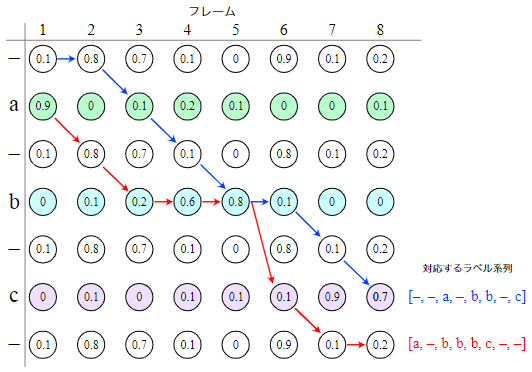
\includegraphics[width=10cm]{./capture/CTC_Frame_Label.png}
  \caption{各フレーム$t$に対する各ラベル$k$の出力確率}
  \label{fig:CTC_Frame_Label}
\end{figure}
$P(l^{\star}|x)$を求めるということは、図\ref{fig:CTC_Frame_Label}の赤や青のパスのような縮約すると$l^{\star}$になるすべてのパスの確率を足し合わせることを意味する。よって
\begin{align}
  P(l^{\star}|x) &= \sum_{\pi \in \mathcal{B}^{-1}(l^{\star})}P(\pi|x)\\
  &= \sum_{\pi \in \mathcal{B}^{-1}(l^{\star})}\prod_{t=1}^{T}y_{t,\pi_t}
\end{align}
と計算できる。前向き・後ろ向きアルゴリズムは、この$P(l^{\star}|x)$を効率的に計算するアルゴリズムである。

\par
ここで、拡張ラベル$\mathbf{l}'=(l'_1, l'_2, \cdots)$を導入する。拡張ラベルは、ラベル系列$l$にブランクトークンを挿入したものである。例えば、$l=[a, b, c]$の場合、拡張ラベルは$\mathbf{l}'=[-, a, -, b, -, c, -]$であり、$l'_1=-, l'_2=a, l'_3=-, l'_4=b, l'_5=-, l'_6=c, l'_7=-$となる。
この拡張ラベルを用いることで、$P(l^{\star}|x)$を以下のように計算できる。
\begin{align}
  P(l^{\star}|x) = \sum_{s=1}^{|l'|} \sum_{\pi \in \mathcal{B}^{-1}(l^{\star}), \pi_t=l'_s} P(\pi|x) \text{ for any }t
\end{align}
この式の、$\sum_{\pi \in \mathcal{B}^{-1}(l^{\star}), \pi_t=l'_s}$の部分の計算のために、前向き・後ろ向きアルゴリズムが用いられる。
\\
\b{前向きアルゴリズム}
\par
始点からフレーム$t$、拡張ラベル$s$に到達するまでの全パスの確率の総和
\begin{align}
  \alpha_t(s) = \sum_{\pi \in \mathcal{B}(\pi_{1:t}) = l_{1:[s/2]}^{\star} } \prod_{t'=1}^{t}y_{t',\pi_{t'}}
\end{align}
\\
\b{後ろ向きアルゴリズム}
\par
フレーム$t$、拡張ラベル$s$から終点まで到達する全パスの確率の総和
\begin{align}
  \beta_t(s) = \sum_{\pi \in \mathcal{B}(\pi_{t:T}) = l_{1:[s/2]}^{\star} } \prod_{t'=1}^{t}y_{t',\pi_{t'}}
\end{align}
例えば、$t=4, s=4$に対しては、
\begin{align}
  \mathcal{B}(\pi_{1:4}) = l_{1:[4/2]}^{\star} = l_{1:2}^{\star} = [a, b]
\end{align}
となる。前向き確率と後ろ向き確率を掛け合わせると、
\begin{align}
  &\alpha_t(s)\beta_t(s) = y_{l'_s}^{t} \sum_{\pi \in \mathcal{B}^{-1}(l^{\star}), \pi_t=l'_s} P(\pi|x)
  &\leftrightarrow
  &P(\pi_t=l'_s|x) = \frac{\alpha_t(s)\beta_t(s)}{P(x)}
\end{align}
となる。従って、損失関数$L$は、上述の$P(\pi_t=l'_s|x)$を用意さえすれば、求めることができる。

\subsection{CTCの運用}
CTCでは推論時に正解ラベル系列が与えられているわけではないため、ある程度割り切って推論を行っていく必要がある。
たとえば、best path decodingという方法は、各フレームごとに最も確率の高いラベルを選択していく方法である。この方法は、シンプルで高速な推論が可能であるが、最適な解を得ることができないという問題がある。


\clearpage
\paragraph{参考文献}
\begin{enumerate}
  \item 岡谷貴之/深層学習 改訂第2版 [機械学習プロフェッショナルシリーズ]/ 講談社サイエンティフィク/ 2022-01-17
  \item 11.スペクトル解析と窓関数 \url{http://www.ic.is.tohoku.ac.jp/~swk/lecture/yaruodsp/win.html}
\end{enumerate}

\newpage
\end{document}